\documentclass[a4paper,11pt]{article}

\usepackage{fullpage}
\usepackage[french]{babel}

\usepackage[utf8]{inputenc}
\usepackage[T1]{fontenc}

\usepackage{mathpazo}
\usepackage{multicol}
\usepackage{url}
%for images
\usepackage{graphicx}
%for code-quoting
\usepackage{listings}
%for pseudo-code algo
\usepackage{algorithm}
\usepackage{algpseudocode}
% Parameters for listings

\lstset{%
  basicstyle=\footnotesize\sffamily,%
  columns=fullflexible,%
  frame=lb,%
  frameround=fftf,%
  language=caml,%
}%

\begin{document}

\begin{titlepage}
  \title{Tours de Hanoï et Pavage de Penrose}
  \author{Guillaume Barbier, Romain Ferrand}
  \date{\today}

  \maketitle

  \begin{abstract}
    
  \end{abstract}
\end{titlepage}

\section*{Introduction}
\begin{center}
	Dans ce document nous allons vous présenter notre étude du problème de Hanoï,
    ainsi que les différentes implémentations visant à sa résolution.
    Puis étudierons différents pavages de Penrose.
\end{center}

\section{Tours de Hanoï}
\label{chap:hanoi}

\subsection{Présentation du problème}
\label{sec:prezHanoi}
\begin{figure}
  \centering
  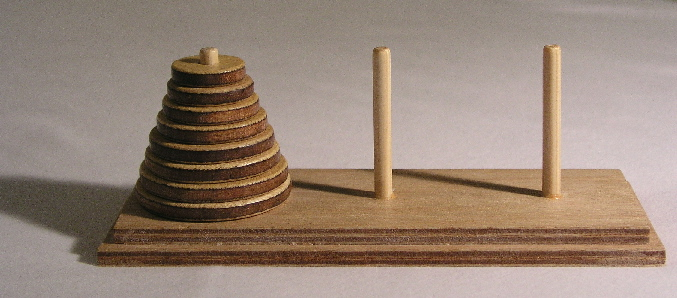
\includegraphics[width=0.8\textwidth]{Tower_of_Hanoi.jpeg}
  \caption{Evanherk wikipédia}
  \label{fig:hanoi}
\end{figure}

Les Tours de Hanoï est un jeu de réflexion inventé par le mathématicien \textbf{Édouard Lucas} (1842-1891).
Il consiste à déplacer un nombre donné de disques de différents diamètre de la tour de départ vers la tour d'arriver,
tout en passant par une tour intermédiaire.

Le joueur doit également respecter deux règles:
\begin{itemize}
\item déplacer un disque à la fois;
\item ne pas déplacer un disque donné sur un disque plus petit.
\end{itemize}

Le nombre de coups optimal pour résoudre les Tours de Hanoï classique est en fonction de $n$ le nombre de disque est : \(\Phi(N) = 2^{N}-1\)

\subsubsection{Implémentation sans affichage graphique}
\label{sec:algoBase}
L'algorithme le plus intuitif pour résoudre le problème des Tours de Hanoï à trois tours,
est un algorithme récursif très simple.

\begin{algorithm}
  \caption{Tours de Hanoï}\label{algo:hanoi1}
  \begin{algorithmic}[1]
    \Procedure{Hanoi}{$disque,src,aux,dest$} \Comment{Trois tours : source, auxiliaire et destination}
    \If{$disque = 0$}
    ne rien faire
    \Else
    \State Hanoi ($disque - 1, src, dest, aux$)
    \State déplacer \textbf{disque} de \textbf{src} à \textbf{dest}
    \State Hanoi ($disque - 1, aux, src, dest$)
    \EndIf
    \EndProcedure
\end{algorithmic}
\end{algorithm}

Il a donc été sans trop difficulté implémenté, avec, dans un premier temps,  un affichage console pour signifier les mouvements effectués.
\begin{lstlisting}
  let rec hanoi (nb_disc:int) (a:rod) (b:rod) (c:rod) =
    if nb_disc = 0 then ()
    else
      begin
        hanoi a c b (n_disc-1);
        movement a c;
        hanoi b a c (n_disc-1)
      end
  ;;
\end{lstlisting}

Nous avons simplement défini un tour par un nouveau type \textbf{rod}, qui dans cette première implémentation est une lettre.

\subsubsection{Validation}

Comme expliqué précédemment l'implémentation basique de Hanoï (de manière récursif) est simple et connue.
Une preuve de son efficacité se démontre par le fait que :
Pour une pile de $N$ disques, pour tout $n$ pile tel que $n \in [1,...,N]$ on effectue $n-1$ déplacement de A vers B puis un déplacement de A vers C puis $n-1$ on a donc bien $2^{N} - 1$ coups effectués.

Le graphique suivant montre le nombre de coup effectués expérimentalement par l'algorithme en fonction du nombre de disques :
\begin{figure}[h]
  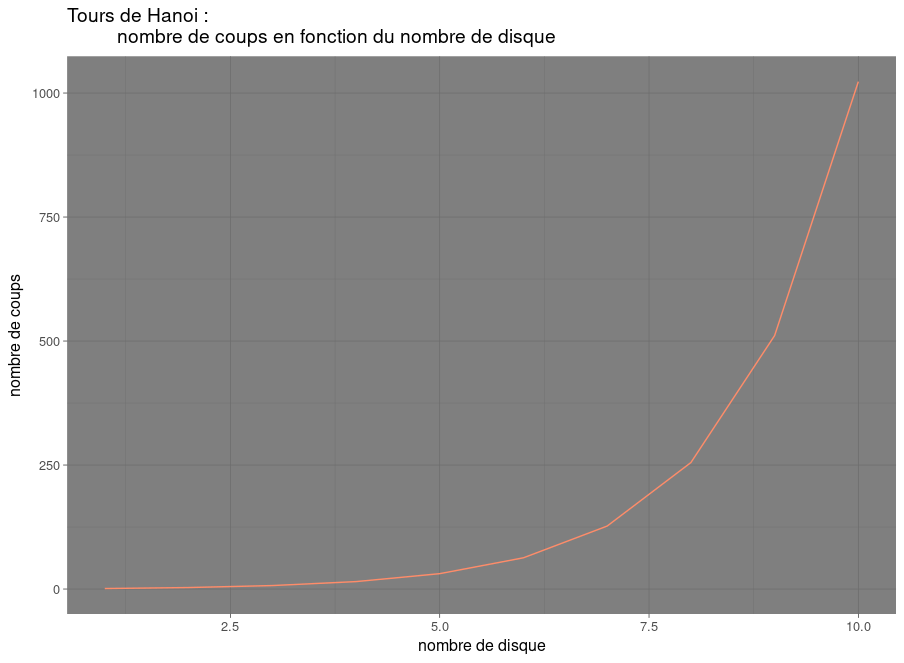
\includegraphics[width=0.8\textwidth]{graph_hanoi.png}
  \label{fig:graph_hanoi}
\end{figure}

\subsection{Implémentation avec affichage graphique}
Dans le cas des tours de Hanoï, nous avons implémenté la première extension proposée à savoir un affichage graphique.
Dans notre implémentation nous avons souhaité afficher à la fois les piquets et les disques.

Notre première approche a été de considérer les types suivants :
\begin{multicols}{3}
\begin{description}
\item[type :] Disque 
	\begin{itemize}
	\item hauteur
	\item largeur 
	\end{itemize}
\item[type :] Contenu piquet
	\begin{itemize}
	\item liste de disque
	\end{itemize}
\item[type :] Forme piquet
	\begin{itemize}
	\item couleur
	\item rectangle (4 points) 
	\end{itemize}
\item[type :]Position piquet
	\begin{itemize}
	\item point 
	\end{itemize}
\item [type :] Piquet 
	\begin{itemize}
	\item position
	\item forme
	\item contenu 
	\end{itemize}
\end{description}
\end{multicols}
\paragraph{De bonnes relations entre les données:}\mbox{}\\
La pile de disque est vu comme ayant une relation de combinaison avec les piquets, ainsi chaque piquet "possède" sa pile de disque et l'affiche en fonction de sa position.
L'idée étant de gérer, par la suite, le déplacement donné par l'algorithme de Hanoï, par un pop du piquet source en push du piquet destination, et de gérer par la suite l'affichage piquet par piquet. 

\paragraph{Mais des problèmes de type:}\mbox{}\\
Dans un premier temps, nous avons implémenté ces types sous forme de tuples, cette manière de faire à rapidement crée un code lourd et complexe à gérer.
En effet, dans le cas du type \textbf{Piquet}, nous devions réfléchir de manière positionnelle ou utiliser l'unpacking de Ocaml, tout en utilisant à la fois que la partie du tuple qui était nécéssaire, nous avions donc a traité plus de données que nous en avions besoin.
Dans un même temps le "champ" \textit{contenu} du type \textbf{piquet} était immutable,
cela se caractérisait par la nécessité de reconstruire une instance de \textbf{piquet} à chaque modification de sa liste de disque.
\paragraph{Et des solutions:}\mbox{}\\
Nous avons donc décidé de remplacer le tuple de \textbf{piquet} par un record, tout en rendant mutable le champ contenu.
Cette manière de faire à permis de clarifier énormément le code, puisque grâce à l'opérateur de résolution 
de portée ".", nous avions un moyen simple de spécifier le lien entre les données.
Cela a permit également de simplifier le code, puisque nous avions plus besoin de réfléchir en terme de position ou d'unpacking, et la liste mutable de disque nous permettait de ne pas avoir à recrée des instances de type \textbf{piquet}.


\section{Retours sur le code}
Dans la première évaluation du code, nous avons reçu plusieurs remarques sur la modularité du code, l'utilisation de structures non pertinentes, etc.
Dans cette partie nous allons vous présenter nos réponses à ces remarques, mais également de optimisations de code que nous avons effectué ou que l'ont aurait pu effectuer.

\paragraph{Optimisations du code:} \mbox{}\\\\
\textbf{Suppression des match with}\\
Que se soit sur le code Hanoï standard ou sur Hanoïextended, nous utilisions le pattern matching de Ocaml alors que cela n'était pas justifié, nous avons remplacé certains de nos  \textbf{match with} par des \textbf{if-else}.
Et nous avons en-capsulé l'utilisation de ceux qui nous semblait les plus justifié dans des modules, dont nous allons vous faire la présentation.\\\\
\textbf{Modification de type forme:}\\
Lors de la précédente implémentation le type \textbf{forme piquet} à été conçu comme un tuple d'une couleur et de 4 points, cette représentation est différente du type de \textbf{disque} sans que cela se justifie.
En effet comme nous stockons la position des piquets il aurait été redondant de stocker les points de la forme du piquet calculer en fonction de cette position.
Nous avons donc juger utile de ne garder que sa position, sa hauteur et sa largeur.

\paragraph{Modularité :}\mbox{}\\\\
Une des lacunes principales de notre code était sa non modularité, en effet la première implémentation utilisait explicitement des types basiques (tuples, a' list, entier, etc.), ainsi que des fonctions d'affichage en même temps que des traitement sur les données.
Le choix a été fait de garder seulement quelques constantes et déclarations ainsi que l'agorithme principal.
Le reste à quand à lui été séparé en trois modules:

\subparagraph{Module Disc}
\begin{center}
	\textbf{Signature du module}
	\begin{lstlisting}
	module Disc:
	sig
	  type disc
	  val make_disc: int -> int -> disc
	  val get_width: disc -> int
	  val get_height: disc -> int
	end
	\end{lstlisting}
\end{center}

Ce module gère simplement le type disque, l'utilisateur à donc simplement la possibilité de crée des disques en fonction d'une largeur et d'une hauteur ainsi que retrouver ces informations à partir d'un disque.

\subparagraph{Module Rod}
\begin{center}
\textbf{Signature du module}
\begin{lstlisting}
module Rod:
sig
  
  type rod
  type pos
  type content
  type shape
  type disc
  val make_shape: Graphics.color -> int -> int -> shape
  val get_shape: rod -> Graphics.color*int*int
  val make_pos: int -> int -> pos
  val get_pos: rod -> int*int
  val make_rod: pos -> shape -> content -> rod
  val make_content: int -> int -> int -> content
  val empty_content: unit -> content
  val get_content: rod -> Disc.disc list
  val pop: rod -> disc
  val push: rod -> disc -> unit    
end
\end{lstlisting}
\end{center}
Ce module permet à l'utilisateur de crée des piquets mais également de crée les structures incluses dans les piquets tout en ayant la possibilité récupérer leurs informations en fonction du piquet.
Nous avons également rajouter des fonctions permettant d'utiliser la pile de disque comme une vrai pile.
En résumé ce module s'occupe de la création et de la mise à jour des structures de données du jeu.

\subparagraph{Module Affichage}
\begin{center}
\textbf{Signature du module}
\begin{lstlisting}
module IO_hanoi:
sig
  val init_screen: int -> int -> unit
  val draw_board: Rod.rod list -> unit
end
\end{lstlisting}
\end{center}
Ce module gère simplement l'affichage en initialisant la fenêtre et en dessinant un état du jeu.
\\
Cette modularité donne à notre code une lisibilité maximale tout en ayant pas d'approprier ni même de connaissance sur l'implémentation interne des objets que nous utilisons.
Ainsi si nous pouvions par la suite une meilleur représentation des données nous pourrions modifier en profondeur certaines module sans que le code principal soit altéré.


\paragraph{Optimisations d'affichage:}\mbox{}\\\\
Notre implémentation va a chaque mouvement, nettoyer la fenêtre et tout réafficher.
Si cette implémentation du code semble peu optimale par rapport à un remplacement par un carré rectangle sur la précédente position du disque.
Elle se justifie par la présence des piquets, qui nécéssite donc l'affichage d'un deuxième rectangle de la bonne couleur en fonction du piquet, mais également par le fait que cette optimisation ne justifie sans doute pas la complexification du code au regard de la simplicité des opérations effectuées.
\subparagraph{}
Une seconde optimisation cette fois effectué a été d'utiliser le double buffering du module Graphics:
Graphics par défaut "dessine" à la fois sur l'écran et dans une zone mémoire appelé backing store.
Grâce à l'option \textbf{autosynchronize false}.
Nous avons pu faire en sorte que graphics écrive que dans le "backing store" et qu'il se synchronise avec l'affichage que lorsqu'on le juge utile, à savoir lorsque toutes les opérations d'affichage ont été effectuées.
Cette manière de faire permet d'éviter les problèmes de \textit{flickering} même lorsque la vitesse du jeu est très rapide.
\subsection{Conclusion sur Hanoï}
Dans le problème des tours de Hanoï, la véritable difficulté a été l'affichage. 
En effet comme l'agorithme est assez intuitif il a été rapidement implémenté.
Sur l'implémentation de l'affichage les difficultés on été sur la clairetté du code et le choix utiliser.
En finalité la version actuelle du code est de bien meilleur qualité puisqu'elle est modulable et permettrait très facilement d'écrire l'algorithme de frame-stewart sans qu'aucune modification soit a faire dans les modules utilisés.

Pour ce qui est des extensions possible une implémentation et étude de cet algorithme est sans doute ce qui manque à notre projet.
 
\end{document}